\section{JavaCraft's Workflow} \label{section: javacraft workflow}
In order to fully understand the mechanism of the game, a flowchart of the entire game is provided below. The flowchart is accompanied by pseudocode.

{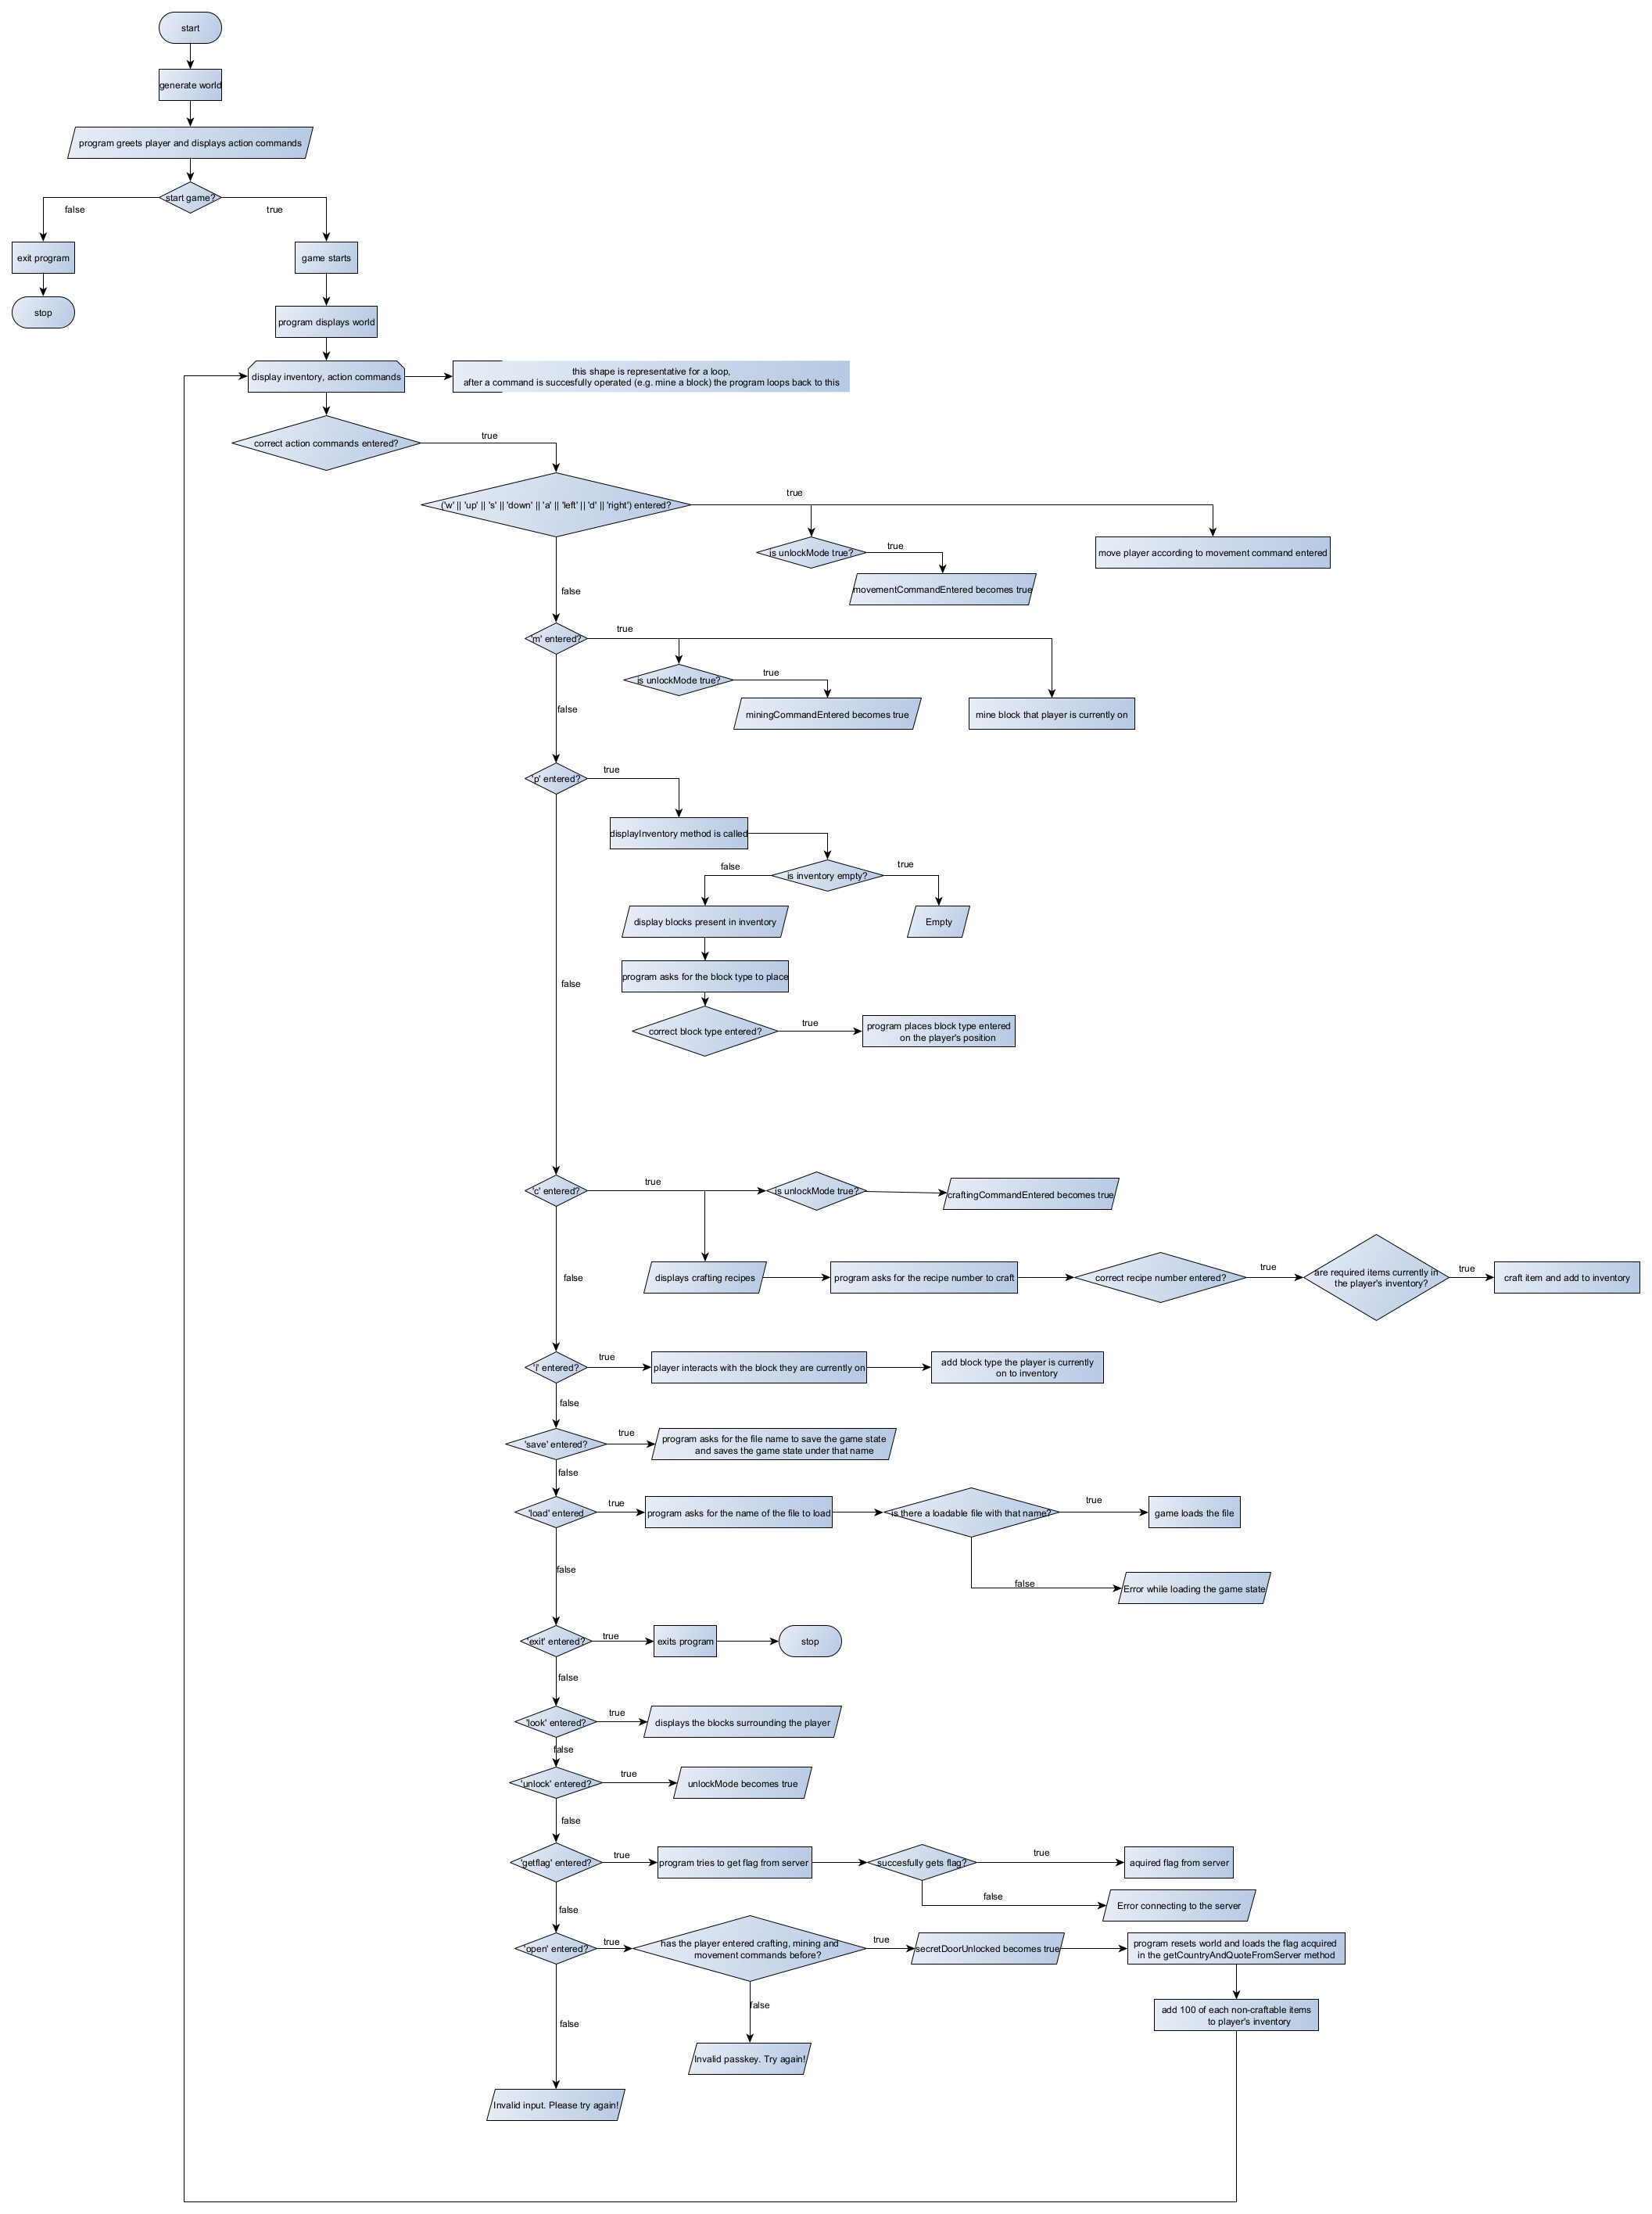
\includegraphics[width=\textwidth,height=\textheight,keepaspectratio]{../flowchart/WorkFlow_of_JavaCraft.png}}

\begin{lstlisting}
    generate world
    print welcome message and instructions
    ask player if they want to start the game
    if choice is equal to 'y' then start game 
       clear screen
       display world
    
       loop
       display inventory, display legend
    
       if input is 'wasd' then move player accordingly 
          if unlockMode is true then movementCommandEntered becomes true
    
       else if input is 'm' then mine the block the player is currently standing on
          if unlockMode is true then miningCommandEntered becomes true
    
       else if input is 'p' then function displayInventory and ask player which block they want to place                                               	if inventory is empty display "Empty"
        else display inventory
          if input is correct then place block on the player's current position
          else inform player they do not have that specific block in their inventory
    
       else if input is 'c' then display crafting recipes 
          ask for recipe number in order to craft 
              if input is correct then check whether the player has the items necessary for the crafting recipe
                  if the player has the necessary items then proceed crafting and add the item to the player's inventory
                  else inform the player they have insufficient resources to craft
          if unlockMode is true then craftinCommandEntered becomes true
       
       else if input is 'i' then player interacts with the block they are currently standing on
          if the block they are currently on is not air then add the item to their inventory
    
       else if input is 'save' then ask player for a name for the current state file they want to save
          save file
    
       else if input is 'load' then ask player for the name of the file they want to load
          if there is a file with that name then load file
          else inform player there has been an error loading the game state
    
       else if input is 'exit' then exit program
    
       else if input is 'look' then inform the player of the block types surrounding them
    
       else if input is 'unlock' then unlockMode becomes true
       
       else if input is 'getflag' then try to get flag from the server
          if unsuccesful then inform the player that there has been an error connecting to the server
    
       else if input is 'open' then check if the booleans craftingCommandEntered, movementCommandEntered, miningCommandEntered true
          if they are true then secretDoorUnlocked becomes true 
             reset world
             load flag world
             add 100 of leaves, stone, iron ore and wood to player's inventory
    
       else inform player that their input is invalid
    end if
    else print "Game not started. Goodbye!" and exit program
    end if
\end{lstlisting}
